\documentclass{article}
\usepackage[utf8]{inputenc}
\usepackage{tikz}
\usetikzlibrary{shapes,arrows}
\usepackage{multicol}
\renewcommand{\contentsname}{{\Huge Table de Matières}}
\usepackage{titlesec}
\titleformat{\section}{\huge\bfseries}{\thesection}{1em}{}
\titleformat{\subsection}{\LARGE\bfseries}{\thesubsection}{1em}{}
\begin{document}
%first page
\begin{center}
\pagenumbering{gobble}
\linespread{2.0}\selectfont

{\Huge U}{\huge NIVERSITÉ DE }{\Huge M}{\huge ONTPELLIER}\\
{\huge L3}{\LARGE ~INFORMATIQUE }
\\~\\~\\~\\~\\
{\Large\textbf{CORRECTEUR DE NOTATION PGN}}
\\~\\~\\~\\~\\

\linespread{1}\selectfont

RAPPORT DE PROJET T.E.R\\
PROJET INFORMATIQUE HLIN601\\
\vfill
\end{center}
\begin{multicols}{2}
\begin{flushleft}
\textbf{Etudiants:}\\
~~M. Jonathan Bazire\\
~~M. Benjamin Baska\\
~~M. Kevin Lastra
\end{flushleft}
\columnbreak
\begin{flushright}
\textbf{Encadrante:}\\
~~Mm. Sylvain Daudé
\end{flushright}
\end{multicols}

\newpage
%bilan
\pagenumbering{arabic}
\setcounter{page}{1}
\tableofcontents
\newpage
%introduction
\section{Introduction}
%{\textbf{\Huge Introduction}}\\~\\~\\
~~Sous la direction de M. Sylvain Daudé, notre groupe composé par Jonathan Bazire, Benjamin Baska et Kevin Lastra à travaillé dans le développement d'u correcteur de notation PGN comme projet du module HLIN601.
\\~\\
Ce projet a pour objectif ......

\newpage
%cahier de charges
\section{Organisation du projet}
\subsection{Objectifs et cahier de charges}
bla bla bla bla bla bla bla bla bla bla bla bla bla bla bla bla bla bla bla bla bla bla bla bla bla bla bla bla bla bla bla bla bla bla bla bla bla bla bla bla bla bla bla bla bla bla bla bla bla bla bla bla bla bla bla bla bla bla bla bla bla bla bla bla bla bla bla bla bla bla bla bla bla bla bla bla bla bla bla bla bla bla bla bla bla bla bla bla bla bla bla bla bla bla bla bla
\begin{figure}[!h]
\centering
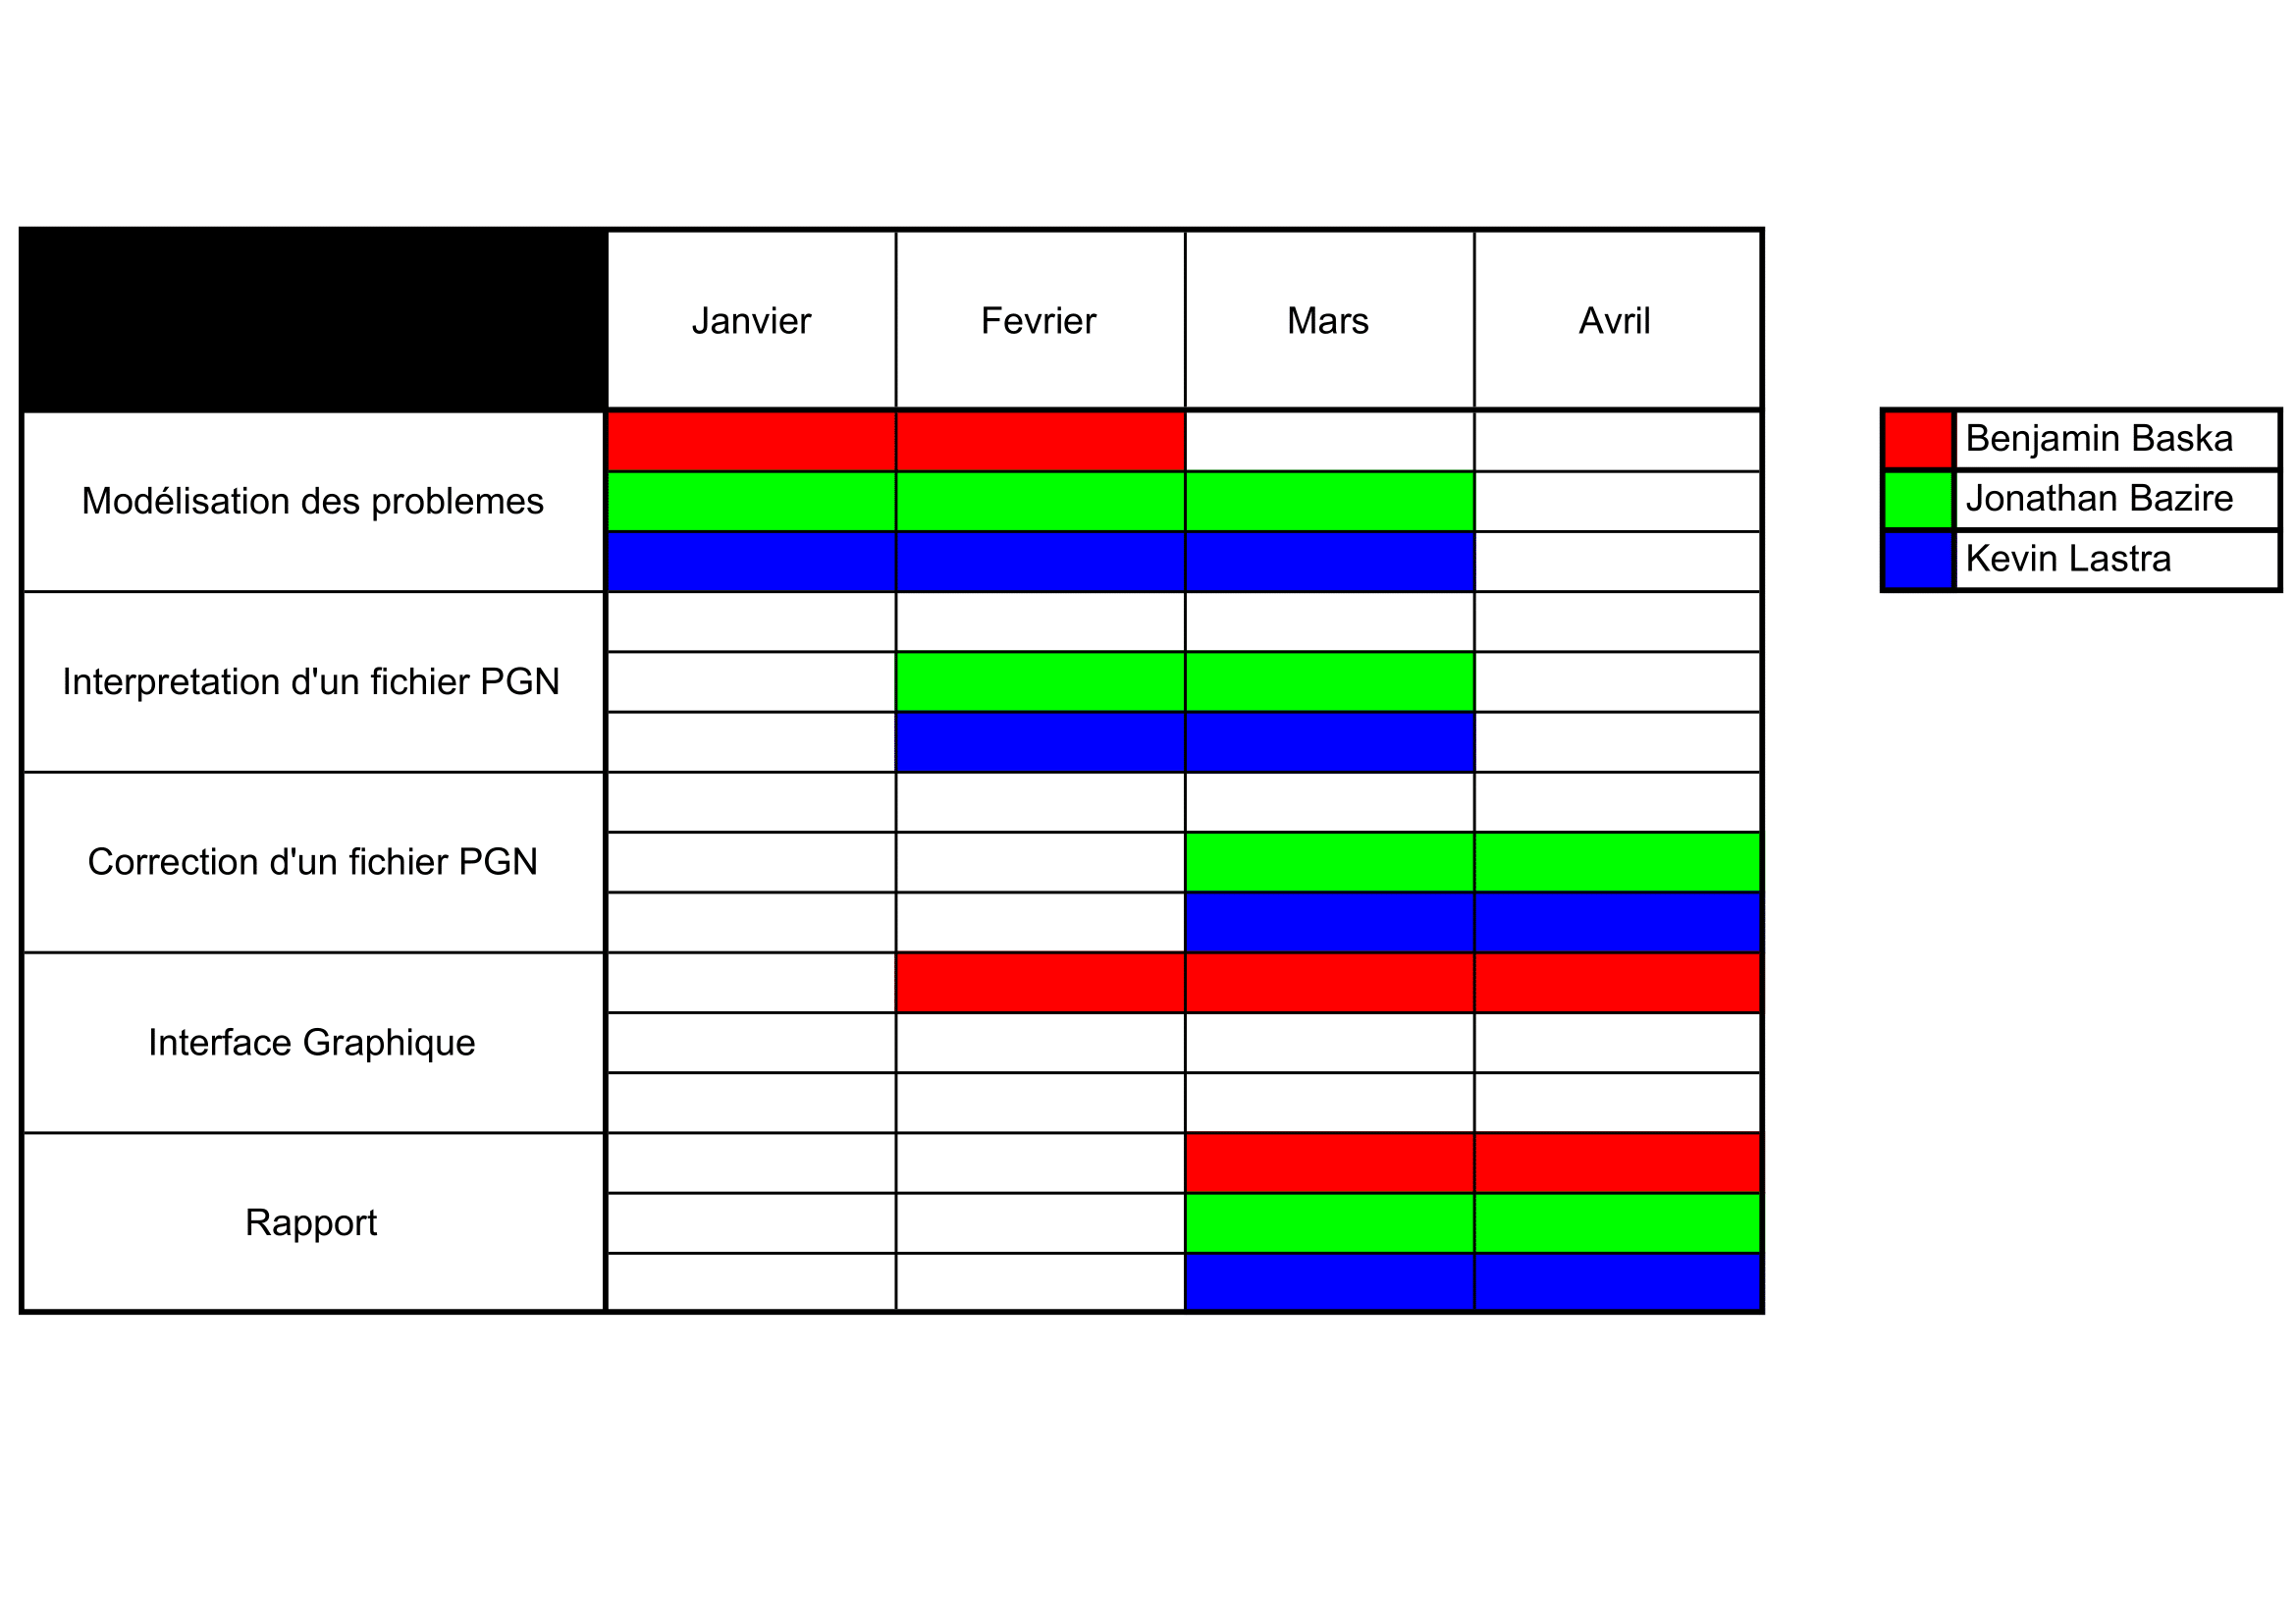
\includegraphics[scale=0.15]{Images/Graph01.png}
\caption{Diagramme de Gantt}
\end{figure}
\newpage
\subsection{Technologies}
~\\~\\
\textbf{\large Langage de programmation et outil de modélisation graphique}
\\~\\
Au début on a choisit de suivre les pas du groupe qui a travailler l'année dernier sur ce projet on utilisent le langage c++ pour le calcul du pgn et javascript, html et php pour le serveur et l'interface graphique, pour avoir a la fin une application web, mais a la fin on c'est décider de tout faire avec le langage c++ et avec l'aide QT, un framework orienter object pour le développement programme avec interface graphique, pour avoir un application sur ordinateur, cette décision a notre point de vue nous economise du temps sur la construction d'un serveur dédie pour l'application, mais surtout parce que c++ et un langage qu'on beaucoup utiliser au long de ces 3 année et aussi parce que QT c'est un application qu'on a déjà manipuler dans le TER de l'année dernier.
~\\~\\
\textbf{\large Travaille collaboratif}
\\~\\
Nous avons utilisé principalement 2 programmes pour pouvoir travailler a distance de la meilleur façon:
\begin{enumerate}
\item GitHub. Ce gestionnaire de version nous permet de partager les avancements du travail réalisé par chacun depuis différents ordinateurs et aussi de sauvegarder plusieurs versions du travail, ce qui est rassurant en cas de perte. 
https://github.com/kevinlastra/TER
\item Discord. Celui-ci nous permet le partage d'écran, la communication orale et écrit, ce qui est utile pour le développement du programme.
\end{enumerate}
\section{Conception}
\section{Bilan et Conclusion}
\section{Bibliographie}
\section{Annexes}
\end{document}